% Options for packages loaded elsewhere
\PassOptionsToPackage{unicode}{hyperref}
\PassOptionsToPackage{hyphens}{url}
%
\documentclass[
]{article}
\usepackage{amsmath,amssymb}
\usepackage{iftex}
\ifPDFTeX
  \usepackage[T1]{fontenc}
  \usepackage[utf8]{inputenc}
  \usepackage{textcomp} % provide euro and other symbols
\else % if luatex or xetex
  \usepackage{unicode-math} % this also loads fontspec
  \defaultfontfeatures{Scale=MatchLowercase}
  \defaultfontfeatures[\rmfamily]{Ligatures=TeX,Scale=1}
\fi
\usepackage{lmodern}
\ifPDFTeX\else
  % xetex/luatex font selection
\fi
% Use upquote if available, for straight quotes in verbatim environments
\IfFileExists{upquote.sty}{\usepackage{upquote}}{}
\IfFileExists{microtype.sty}{% use microtype if available
  \usepackage[]{microtype}
  \UseMicrotypeSet[protrusion]{basicmath} % disable protrusion for tt fonts
}{}
\makeatletter
\@ifundefined{KOMAClassName}{% if non-KOMA class
  \IfFileExists{parskip.sty}{%
    \usepackage{parskip}
  }{% else
    \setlength{\parindent}{0pt}
    \setlength{\parskip}{6pt plus 2pt minus 1pt}}
}{% if KOMA class
  \KOMAoptions{parskip=half}}
\makeatother
\usepackage{xcolor}
\usepackage{graphicx}
\makeatletter
\def\maxwidth{\ifdim\Gin@nat@width>\linewidth\linewidth\else\Gin@nat@width\fi}
\def\maxheight{\ifdim\Gin@nat@height>\textheight\textheight\else\Gin@nat@height\fi}
\makeatother
% Scale images if necessary, so that they will not overflow the page
% margins by default, and it is still possible to overwrite the defaults
% using explicit options in \includegraphics[width, height, ...]{}
\setkeys{Gin}{width=\maxwidth,height=\maxheight,keepaspectratio}
% Set default figure placement to htbp
\makeatletter
\def\fps@figure{htbp}
\makeatother
\setlength{\emergencystretch}{3em} % prevent overfull lines
\providecommand{\tightlist}{%
  \setlength{\itemsep}{0pt}\setlength{\parskip}{0pt}}
\setcounter{secnumdepth}{-\maxdimen} % remove section numbering
\ifLuaTeX
  \usepackage{selnolig}  % disable illegal ligatures
\fi
\IfFileExists{bookmark.sty}{\usepackage{bookmark}}{\usepackage{hyperref}}
\IfFileExists{xurl.sty}{\usepackage{xurl}}{} % add URL line breaks if available
\urlstyle{same}
\hypersetup{
  hidelinks,
  pdfcreator={LaTeX via pandoc}}

\author{}
\date{}

\begin{document}

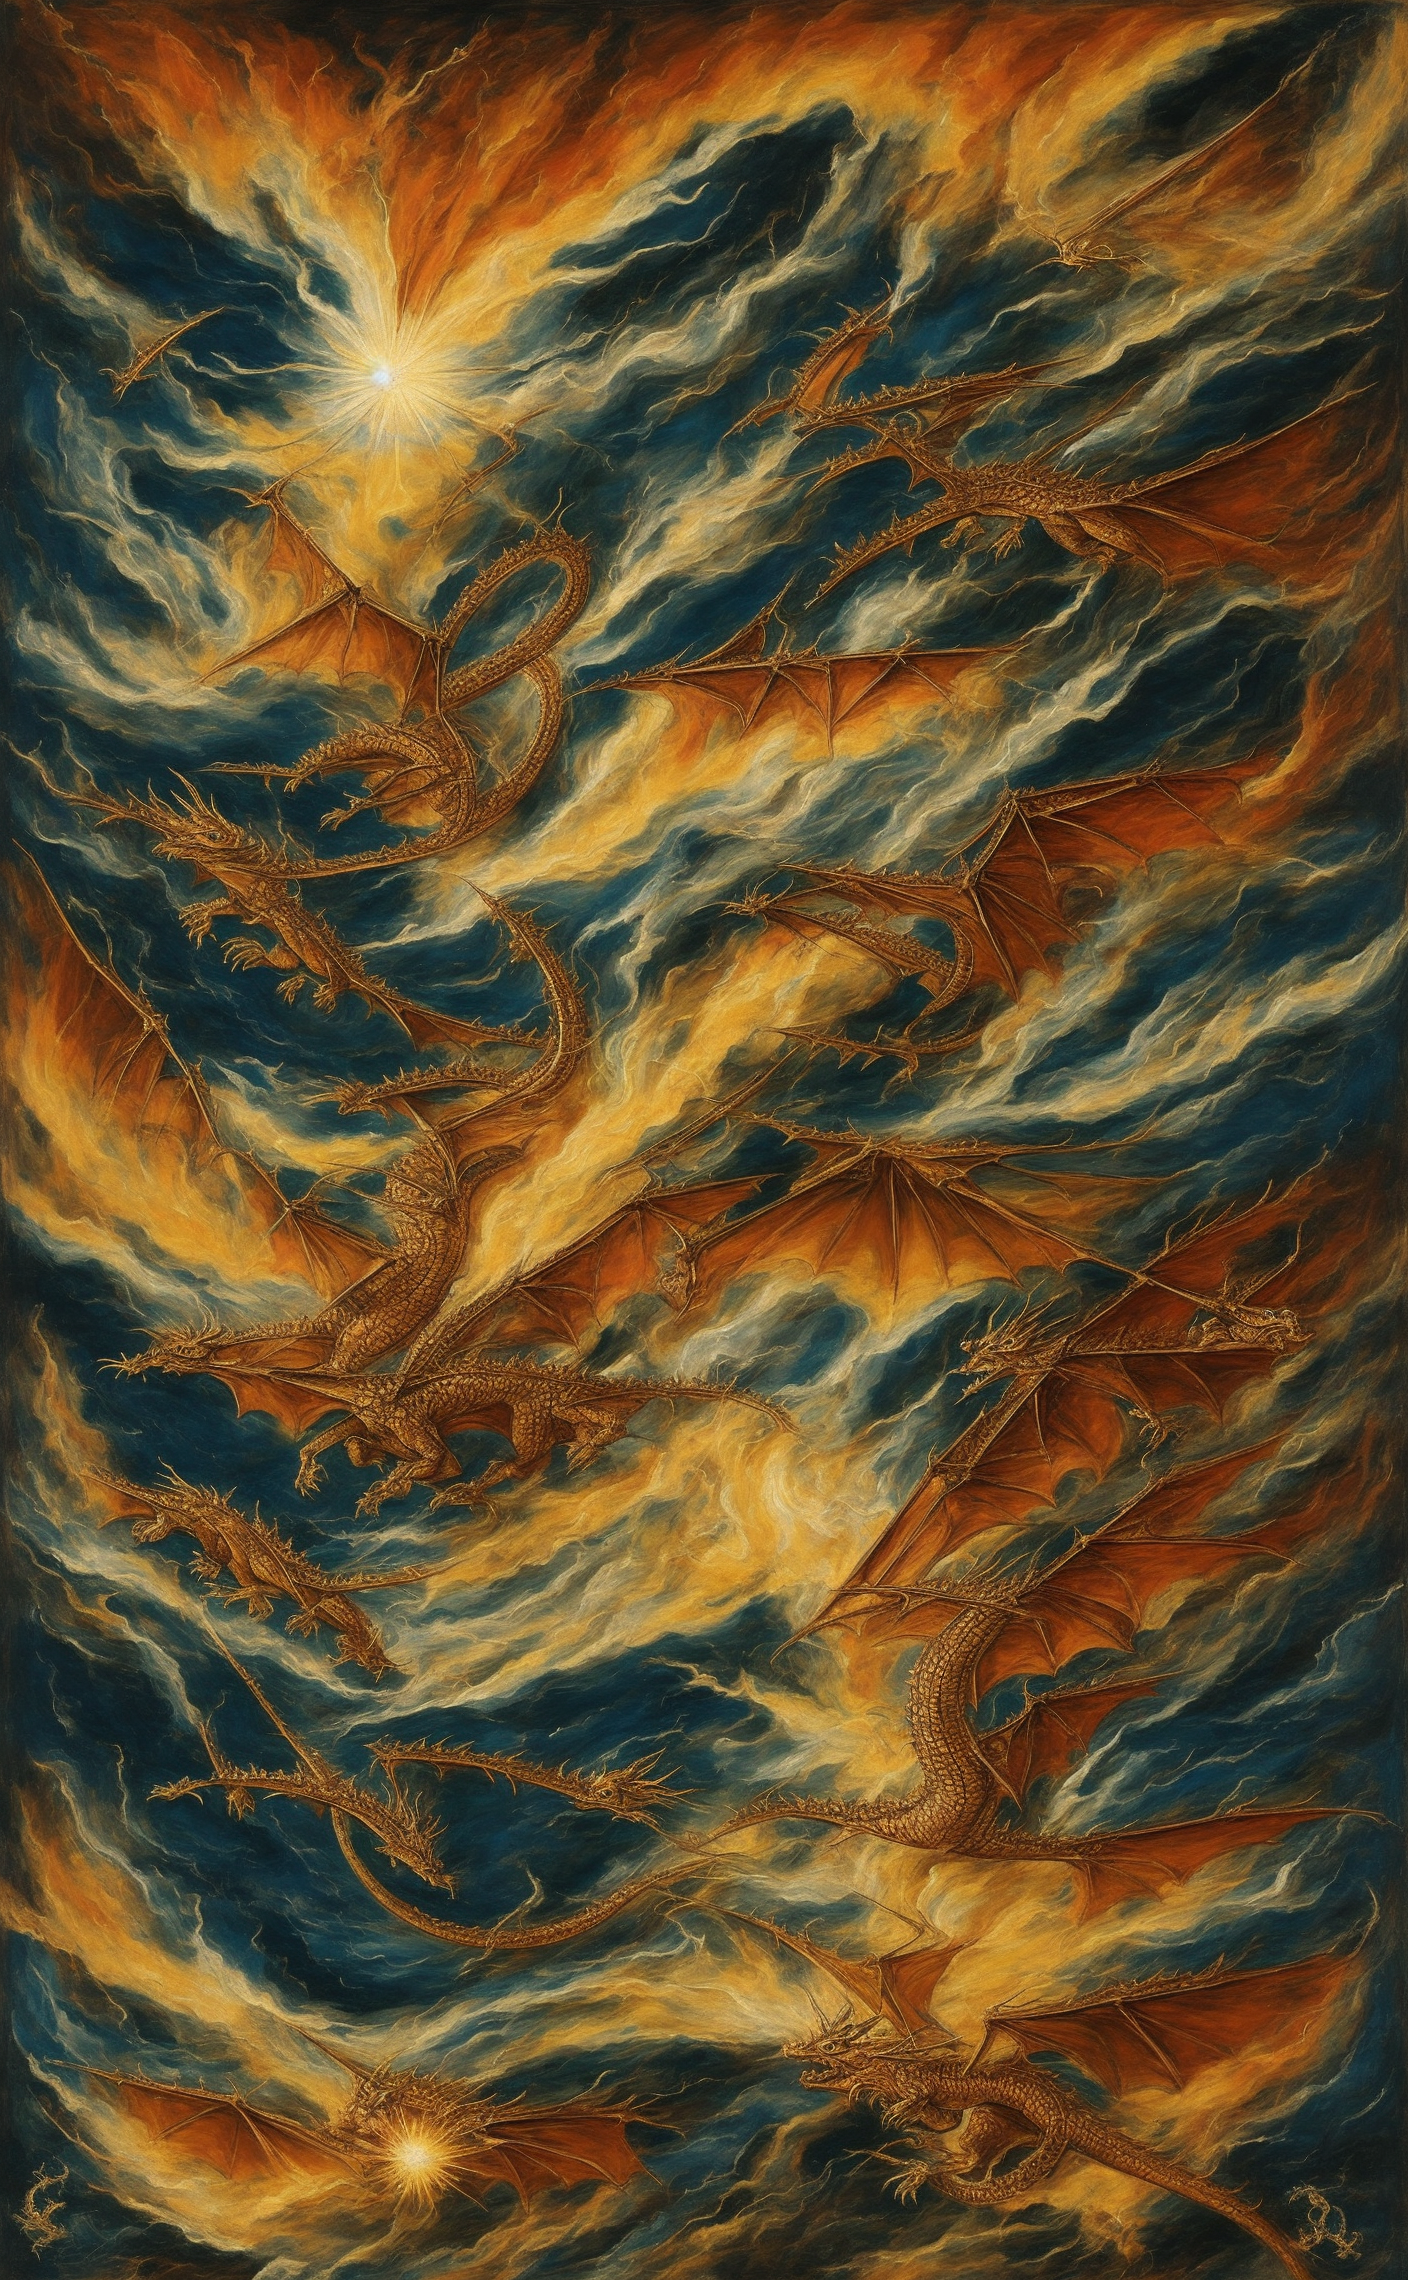
\includegraphics{/home/jw/src/iching_cli/defs/01/01.png}

\section{䷀ Creation}\label{ux4dc0-creation}

\subsection{Core Meaning}\label{core-meaning}

The pure force of origination and initiative. Like heaven generating
existence, this represents the primary creative impulse that initiates
all manifestation.

\subsection{Structure}\label{structure}

\textbf{King Wen Sequence}: 1\\
\textbf{King Wen Title}: Ch\textquotesingle ien (The Creative)\\
\textbf{Binary Sequence}: 63 (111111)\\
\textbf{Above}: Qian (Heaven, Creative Force, Dynamic)\\
\textbf{Below}: Qian (Heaven, Creative Force, Dynamic)\\
\textbf{Perspective}: Pure creative force in action

\subsection{Key Attributes}\label{key-attributes}

\textbf{Nature}: Initiating\\
\textbf{Action}: Manifesting\\
\textbf{Success through}: Strong, persistent creation\\
\textbf{Image}: Heaven in motion; Dragons soaring\\
\textbf{Challenge}: Maintaining wisdom while wielding power

\subsection{Lines in Transition}\label{lines-in-transition}

\textbf{Line 6}: \emph{Transcendent Dragon}: Vision beyond convention;
\emph{Create with wisdom}\\
\textbf{Line 5}: \emph{Flying Dragon}: Creation at its peak; \emph{Act
with confidence}\\
\textbf{Line 4}: \emph{Leaping Dragon}: Growing power; \emph{Prepare for
emergence}\\
\textbf{Line 3}: \emph{Active Dragon}: Creative engagement; \emph{Work
diligently}\\
\textbf{Line 2}: \emph{Dragon in Fields}: Building strength;
\emph{Gather resources}\\
\textbf{Line 1}: \emph{Hidden Dragon}: Potential stirring; \emph{Begin
carefully}

\subsection{Tholonic Analysis}\label{tholonic-analysis}

\subsubsection{Negotiation}\label{negotiation}

The hexagram represents pure creative force, with both trigrams being
Qian/Heaven. This creates unimpeded generative power.

\subsubsection{Limitation}\label{limitation}

Structure is provided by heaven above and below, indicating that
creation follows cosmic principles. The doubled heaven suggests
amplified creative force.

\subsubsection{Contribution}\label{contribution}

This pattern contributes to evolution by initiating new forms. It shows
how consciousness manifests reality through directed will.

\subsubsection{Significance in the
Thologram}\label{significance-in-the-thologram}

In the tholonic system, this hexagram represents pure creative
consciousness. It demonstrates how awareness generates existence through
focused intention.

\subsection{No Moving Lines}\label{no-moving-lines}

When no lines are changing, focus on steady creation. Success comes
through persistent generation rather than forced manifestation.

\subsection{All Moving Lines}\label{all-moving-lines}

A complete transformation in how creation functions is indicated. Old
patterns of manifestation must give way to new forms of generation.
Ensure wisdom guides power while embracing change.\# Three Tales of
"Creation"

\subsection{The Symphony Maker (Man vs.
Man)}\label{the-symphony-maker-man-vs-man}

\emph{In the style of Herman Melville}

In a world where music had been standardized to government-approved
harmonies, Composer Chen built a secret piano that could play the spaces
between notes. Like a whaler pursuing the unseen beneath waves, she
hunted the wild melodies that lived in fractional tones.

Each night in her basement laboratory, surrounded by modified tuning
forks and resonance chambers, she worked to capture sounds no human had
heard before. The authorities called it noise, but those who listened
closely heard the voice of creation itself.

When she finally performed her "Ocean of Stars" symphony, using her
quarter-tone piano, she didn\textquotesingle t just break the rules of
music -- she revealed they had never existed.

\subsubsection{Key Elements:}\label{key-elements}

Line 6: Universal Impact - Redefining the nature of music itself\\
Line 5: Masterwork Creation - The "Ocean of Stars" symphony\\
Line 4: Building Power - Developing the revolutionary instrument\\
Line 3: Persistent Work - Nightly experimentation\\
Line 2: Foundation Building - Creating modified instruments\\
Line 1: Initial Vision - Discovering spaces between notes

\subsection{The Storm Weaver (Man vs.
Nature)}\label{the-storm-weaver-man-vs-nature}

\emph{In the style of Homer}

When the Great Drought threatened to destroy her people, Maria
discovered she could weave clouds from spider silk and morning dew. Like
Athena at her loom, she studied how each strand of moisture caught the
light, how wind patterns could be woven into larger forms.

First came small clouds, no bigger than basketballs, drifting above her
garden. Then came floating rivers of mist, drawn from the
earth\textquotesingle s deepest breaths. Finally, she learned to weave
storm systems that danced across continents.

Nature itself watched in wonder as she created weather patterns ancient
as time yet new as dawn.

\subsubsection{Key Elements:}\label{key-elements-2}

Line 6: Global Impact - Continental weather weaving\\
Line 5: Mastery Shown - Creating storm systems\\
Line 4: Growing Scope - Expanding to floating rivers\\
Line 3: Active Development - Daily weaving practice\\
Line 2: Basic Success - First small clouds\\
Line 1: Initial Discovery - Learning moisture patterns

\subsection{The Dream Architect (Man vs.
Self)}\label{the-dream-architect-man-vs-self}

\emph{In the style of Stanisław Lem}

In 2157, when consciousness augmentation had reached its limits, Dr. Wei
discovered she could build new forms of awareness from pure mathematical
structure. Not expanding the mind, but creating entirely new types of
thought.

She began with simple geometric consciousness -- minds that thought in
perfect squares and circles. Each iteration grew more complex:
consciousness based on wave functions, on prime number sequences, on
fractal patterns that thought about themselves thinking.

When she finally succeeded in creating a mind based on the mathematics
of creation itself, she found she had not built a new consciousness, but
discovered how consciousness had built itself.

\subsubsection{Key Elements:}\label{key-elements-3}

Line 6: Universal Understanding - Discovering
consciousness\textquotesingle s nature\\
Line 5: Peak Achievement - Creating self-recursive awareness\\
Line 4: Complex Development - Building mathematical minds\\
Line 3: Active Experimentation - Testing different thought forms\\
Line 2: Basic Structures - Geometric consciousness\\
Line 1: Foundation Theory - Pure mathematical awareness\#
Tesla\textquotesingle s Vision of Wireless Power

\subsection{"Creation" in History}\label{creation-in-history}

In 1899, Nikola Tesla established his Colorado Springs laboratory to
prove that Earth itself could conduct electrical power. While others
focused on incremental improvements to existing systems, Tesla
envisioned creating an entirely new paradigm of global power
distribution.

In his experimental station, Tesla generated artificial lightning bolts
over a hundred feet long and illuminated light bulbs wirelessly at
distances up to 25 miles. Each experiment built upon the last, leading
to his ultimate vision - the Wardenclyffe Tower project, designed to
transmit power and information wirelessly across the globe.

Though financial constraints prevented the tower\textquotesingle s
completion, Tesla\textquotesingle s creative vision demonstrated
unprecedented scope. He didn\textquotesingle t just improve existing
technology; he attempted to create an entirely new relationship between
humanity and electricity. His Colorado Springs experiments proved that
wireless power transmission was possible, laying groundwork for
technologies we\textquotesingle re still developing today.

\emph{Source: "Tesla: Man Out of Time" by Margaret Cheney (1981) and
"Wizard: The Life and Times of Nikola Tesla" by Marc Seifer (1996)}

\subsubsection{Key Elements:}\label{key-elements-4}

Line 6: Universal Vision - Concept of worldwide wireless power\\
Line 5: Peak Achievement - Successful long-distance power transmission\\
Line 4: Growing Capability - Increasingly powerful demonstrations\\
Line 3: Active Experimentation - Daily testing and refinement\\
Line 2: Foundation Building - Laboratory establishment\\
Line 1: Initial Insight - Recognition of Earth\textquotesingle s
conductive potential

\end{document}
